\section{Process View}
\label{sec_process}

\subsection{Overview}

The purpose of the process view is to specify the non-functional requirements of the software. It describes the concurrency and synchronization aspects of the \textit{libsafecryto} library.

\subsection{Stakeholders}

\textbf{\textit{Developers, Testers}}

\textit{A description of all stakeholders is contained in Section \ref{sec:stakeholders}.}

\subsection{Library Instantiation}

It will be possible during instantiation of the library to enable the use of multithreading in a number of forms:

\begin{enumerate}[(a)]
\item Exploiting parallelism within the cryptographic scheme itself
\item Performing random number generation (including Gaussian Sampling) as a background task
\end{enumerate}

The following diagram (Figure \ref{fig:safecrypto_activity}) describes the typical creation of an instance of the \textit{libsafecrypto} library. During the creation and initialisation phase the information supplied by the user to the Interface Layer is used to define the correct Scheme Layer and configure any global resources resources such as the PRNG, error queue and debugging resources. In turn, the selected cryptographic scheme is created and initialised using the common API to all schemes. All resources associated with the scheme are created including threading resources (threadpools, IPC, etc.), arithmetic, hashing, Gaussian Sampling and memory resources. The API is then used to return a pointer to the created instance that lies on the heap and the relevant error code.

\begin{figure}[H]
\centering
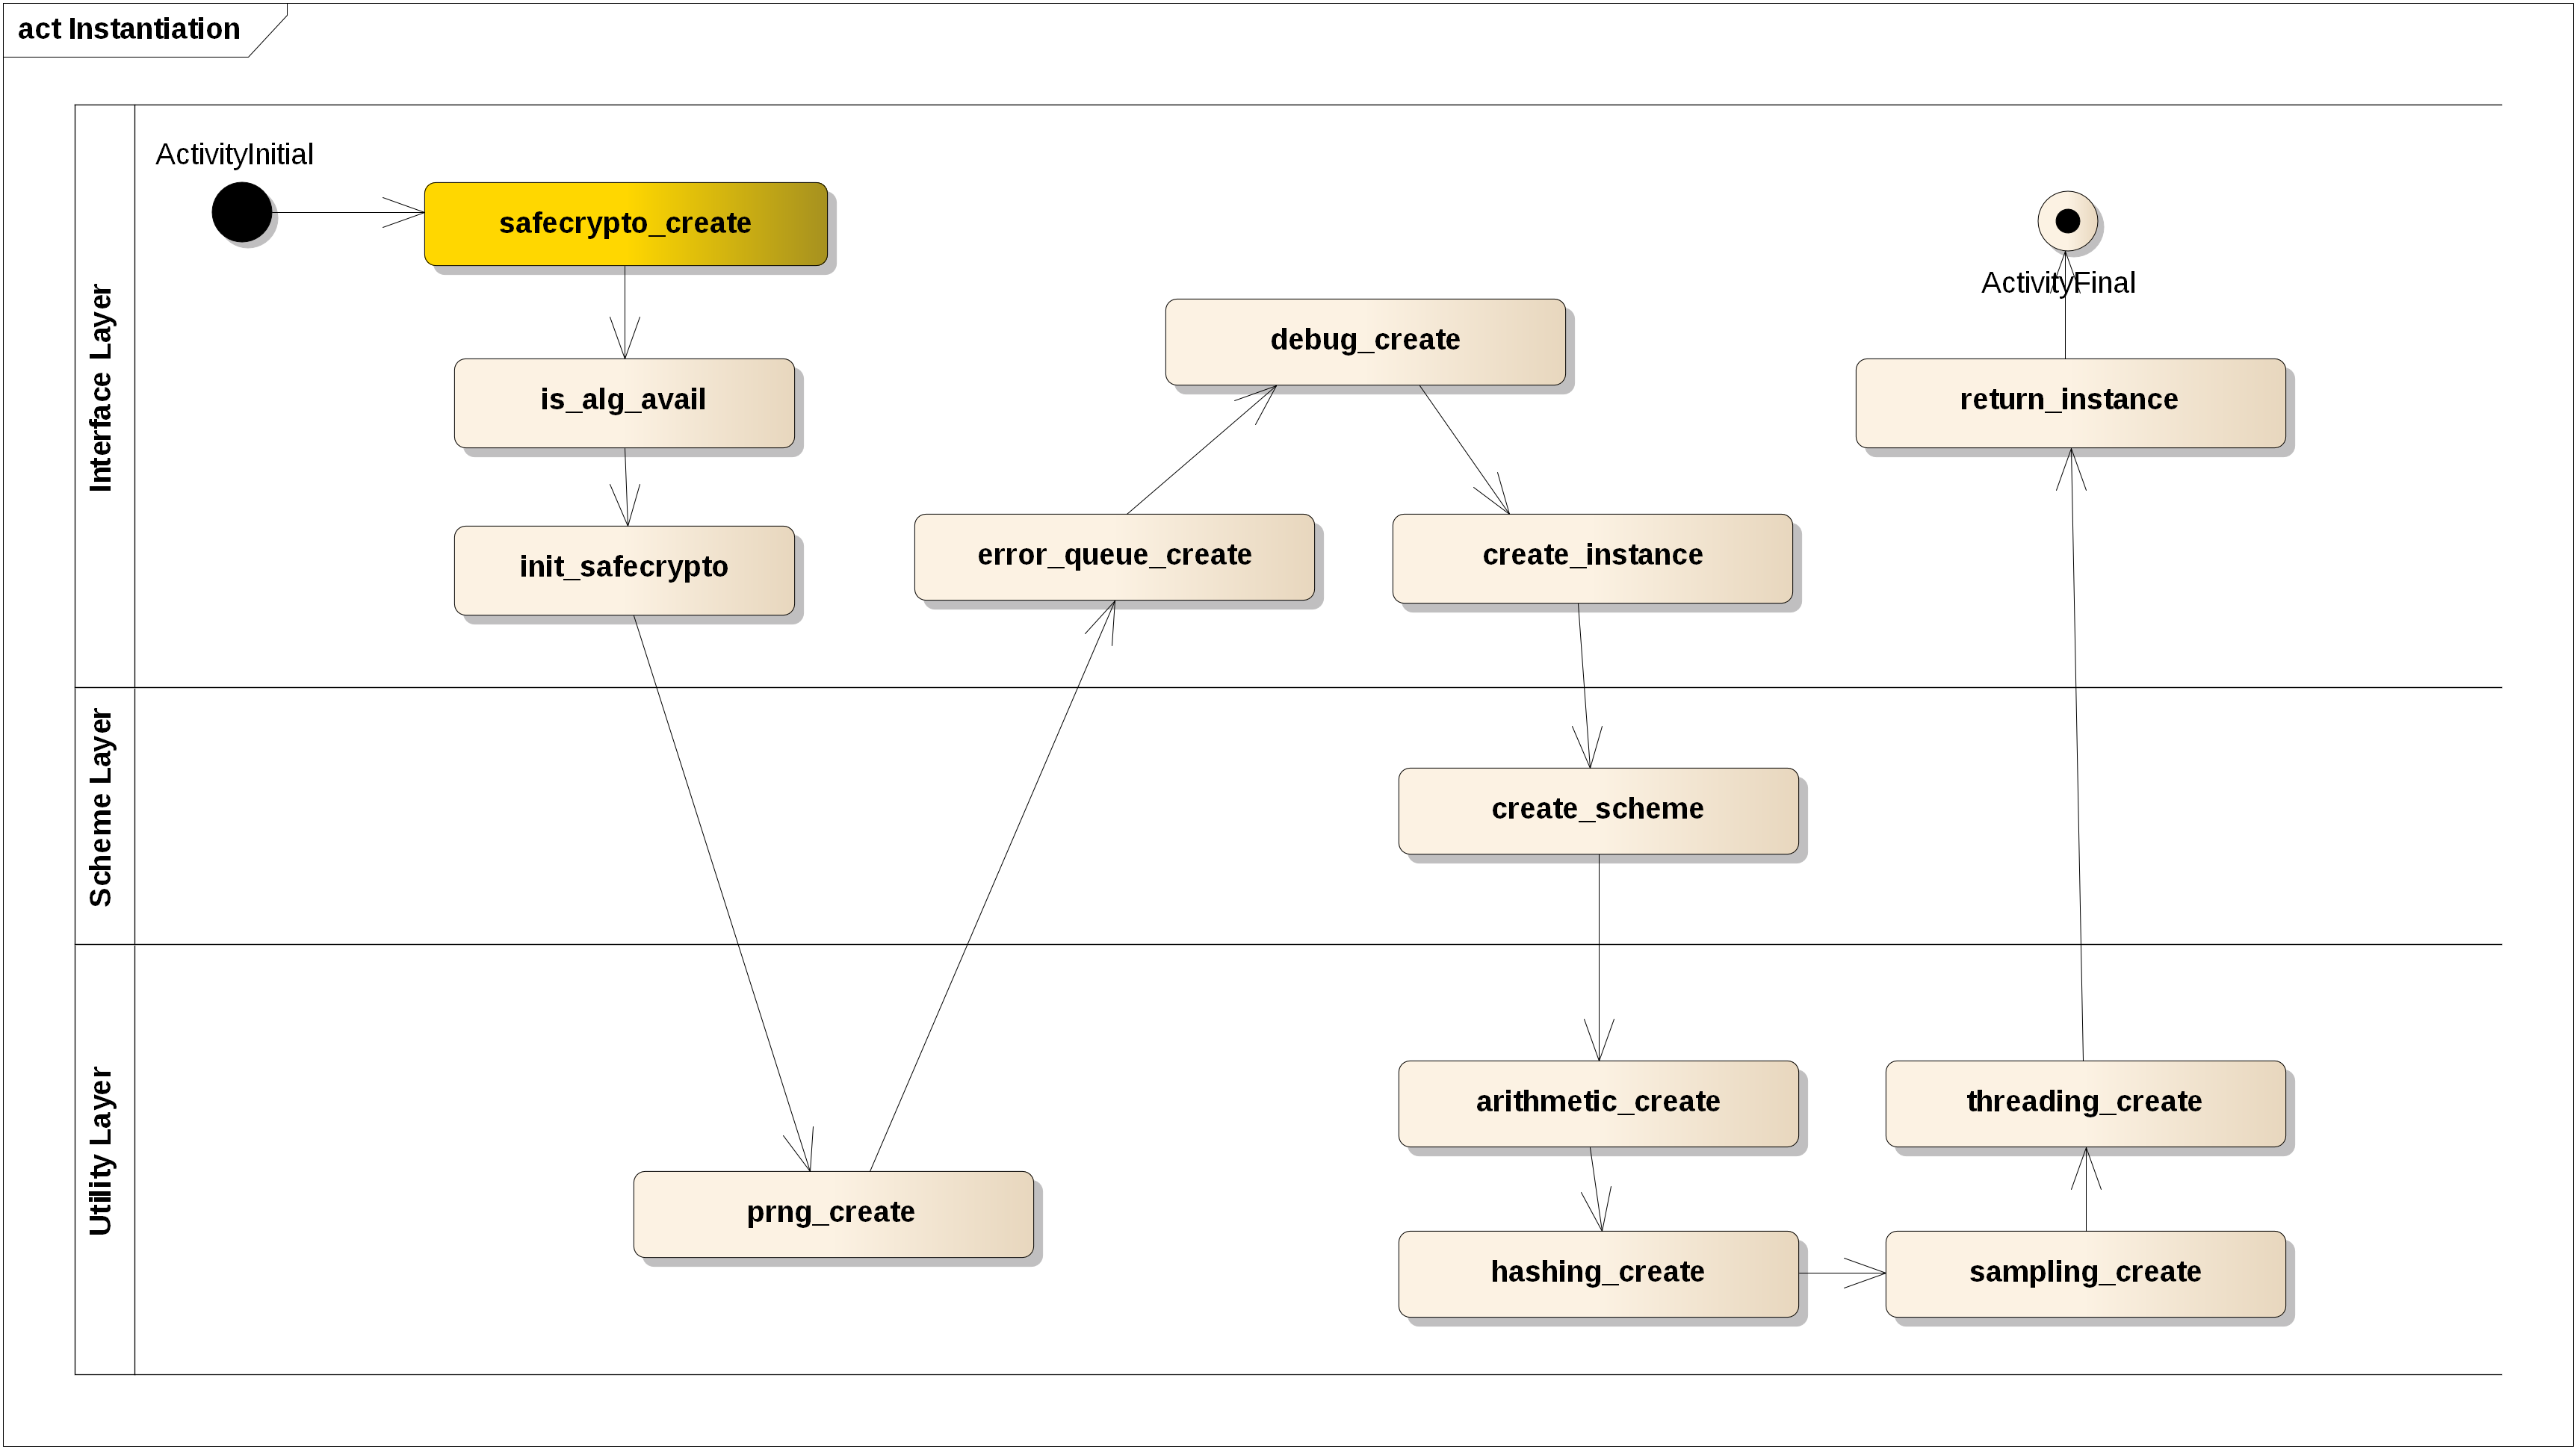
\includegraphics[width=\textwidth]{activity_instantiation.png}
\caption{Activity diagram of the creation of a SAFEcrypto instance}
\label{fig:safecrypto_activity}
\end{figure}


\subsection{Library Destruction}

The destruction of an instance of \textit{libsafecrypto} follows the description provided in Figure \ref{fig:safecrypto_destruct_activity}. All interactions with the API using the pointer to the SAFEcrypto instance are first verified. The destroy function associated with the instantiated cryptographic scheme is then called to ensure that all low-level scheme specific memory and threading resources are relinquished. Following this all global memory resources within \textit{libsafecrypto} are released, this includes the key pair, debug printing, error queue and the SAFEcrypto instance itself.

\begin{figure}[H]
\centering
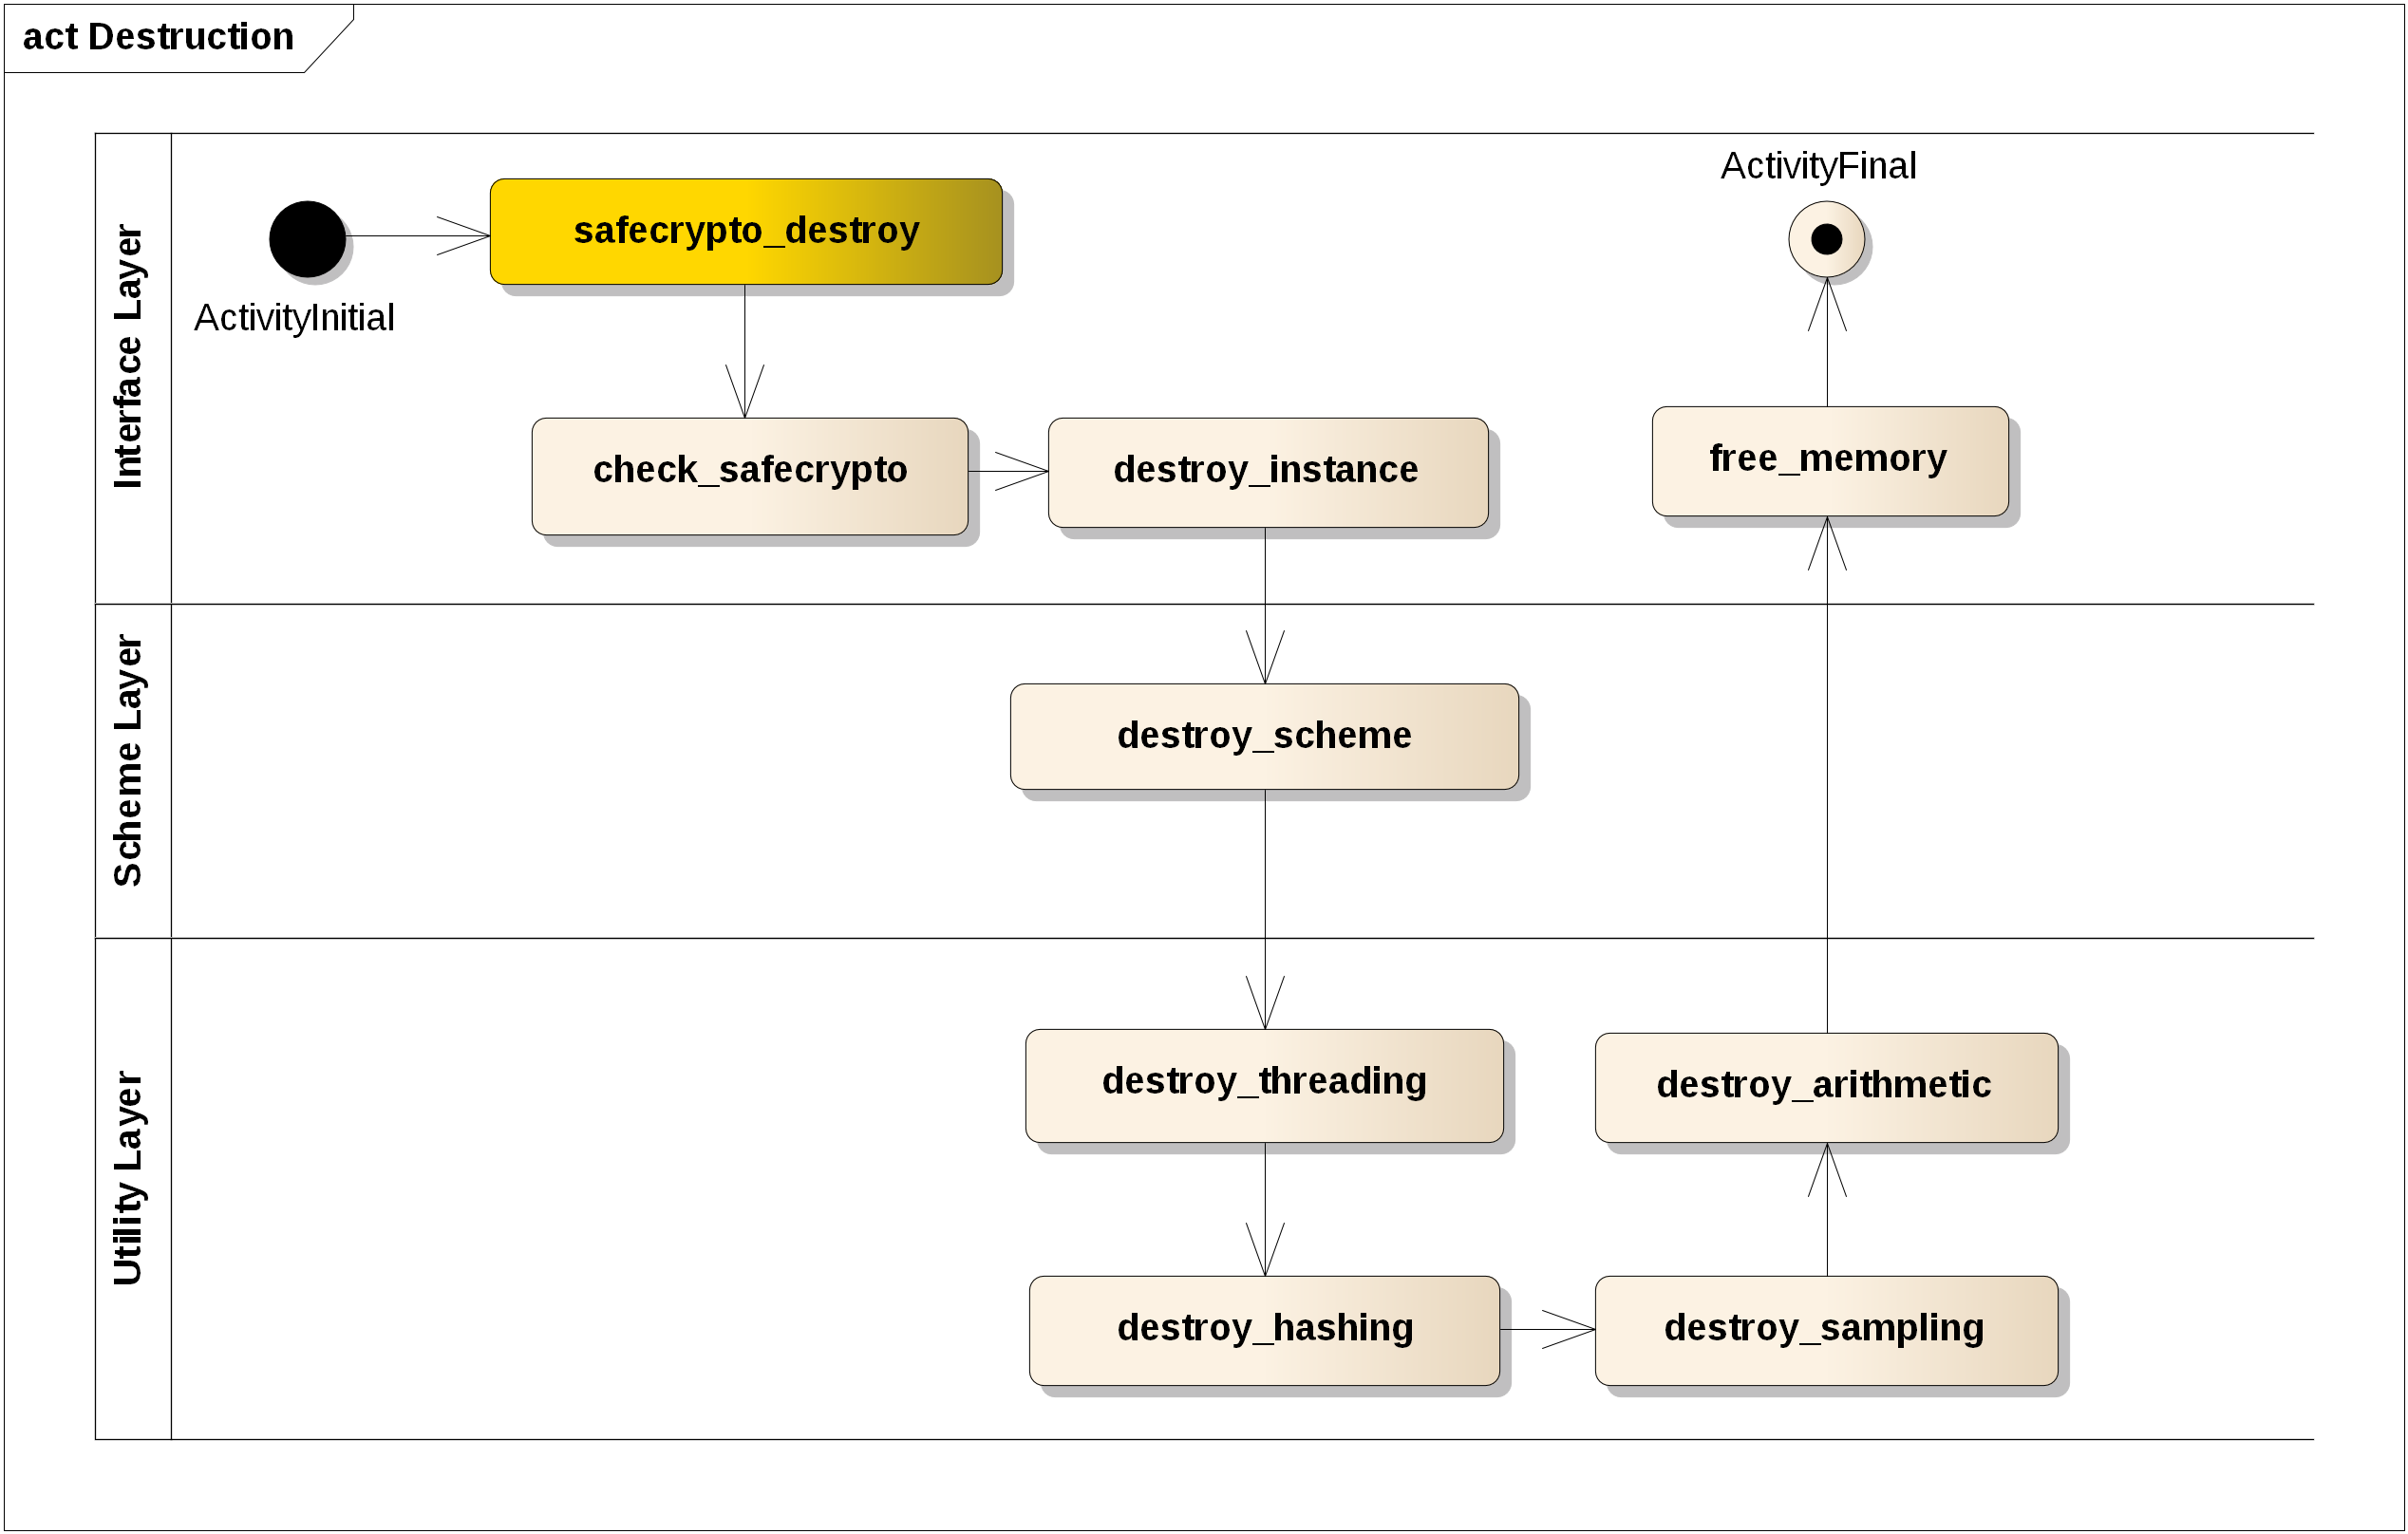
\includegraphics[width=\textwidth]{activity_destruction.png}
\caption{Activity diagram of the destruction of a SAFEcrypto instance}
\label{fig:safecrypto_destruct_activity}
\end{figure}


\newpage
\subsection{Performing a Cryptographic Operation}

As shown in Figure \ref{fig:safecrypto_operation_activity} each cryptographic operation relies upon resources that are created during instantiation of the library such as threadpools and data storage. If multithreading is enabled then a threadpool can be used to perform various tasks for each scheme.

\begin{figure}[H]
\centering
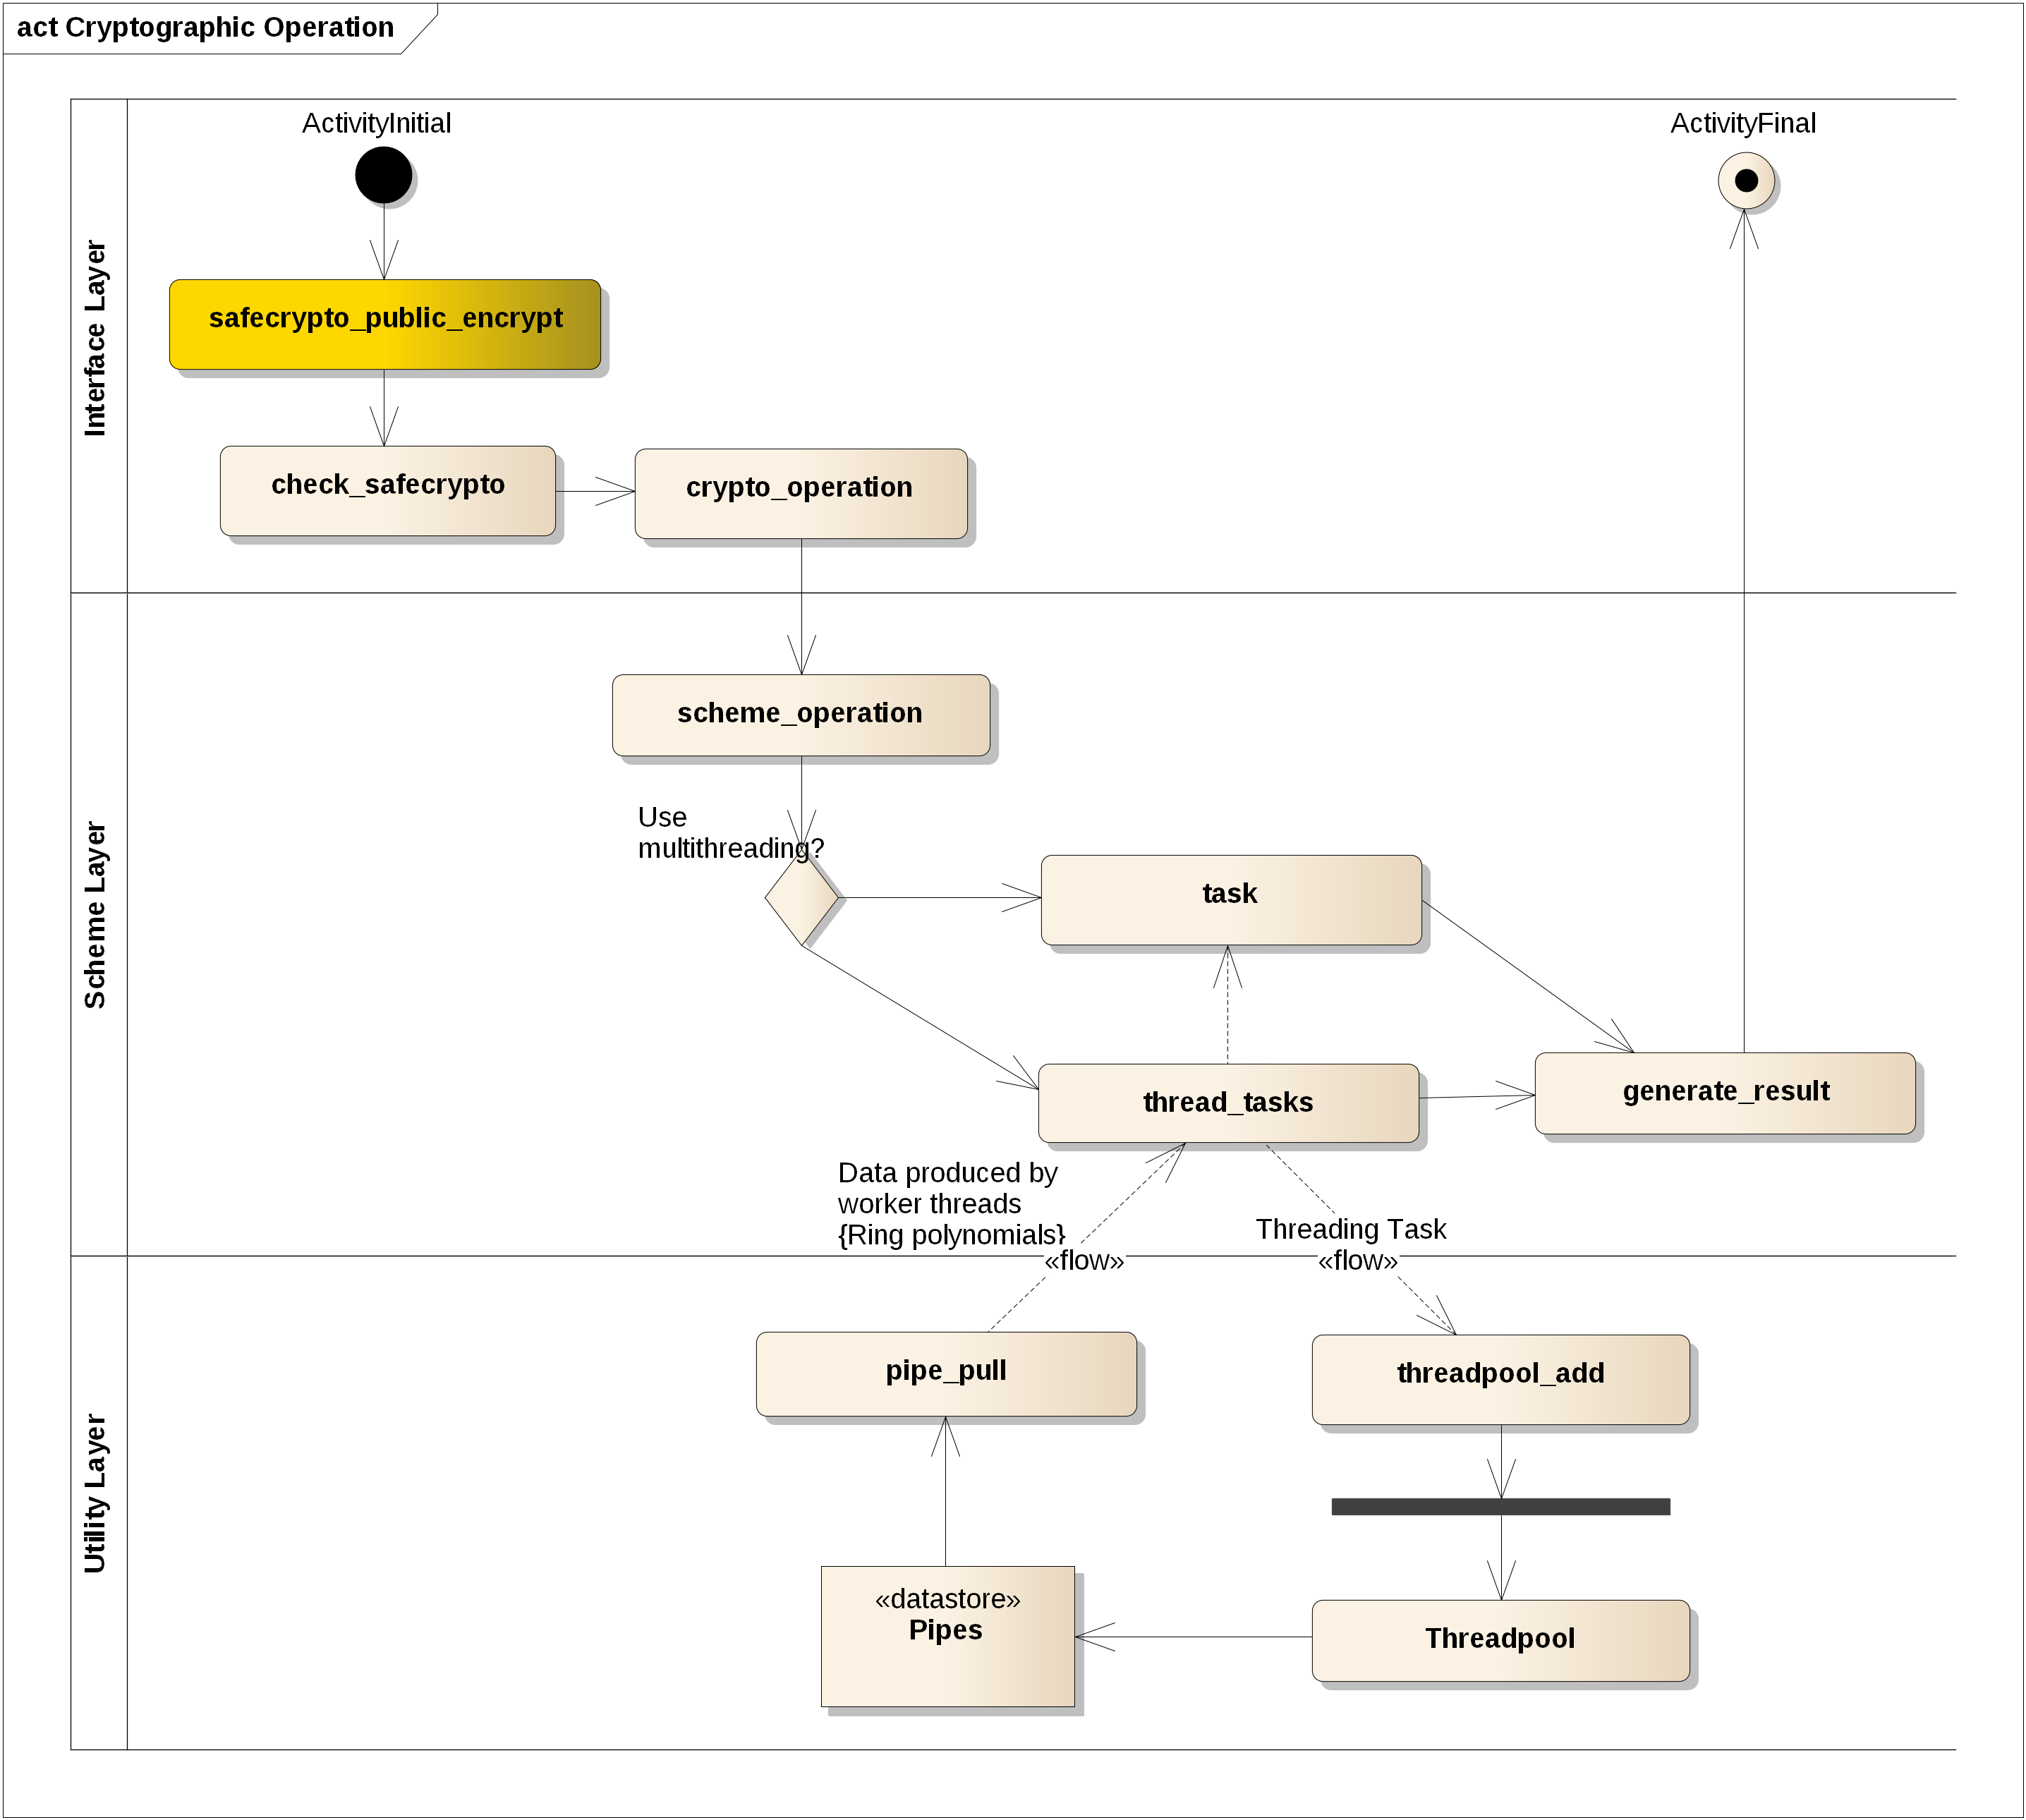
\includegraphics[width=\textwidth]{activity_crypto_operation.png}
\caption{Activity diagram of a SAFEcrypto cryptographic operation}
\label{fig:safecrypto_operation_activity}
\end{figure}


